%!TEX TS-program = xelatex
%!TEX encoding = UTF-8 Unicode

\documentclass[a4paper]{article}

\usepackage{xltxtra}
\usepackage{amsfonts}
\usepackage{polyglossia}
\usepackage{fancyhdr}
\usepackage{geometry}
\usepackage{dsfont}
\usepackage{amsmath}
\usepackage{amsthm}
\usepackage{physics}
\usepackage{float}
\usepackage{tikz}
\usepackage{bm}
\usepackage[shortlabels]{enumitem}
\usetikzlibrary{shapes,arrows,positioning}

\geometry{a4paper,left=15mm,right=15mm,top=20mm,bottom=20mm}
\pagestyle{fancy} \lhead{Devon Morris}
\chead{Detection \& Estimation Theory - Homework 5}
\rhead{\today}
\cfoot{\thepage}

\setlength{\headheight}{23pt}
\setlength{\parindent}{0.0in}
\setlength{\parskip}{0.0in}

\newtheorem{prop}{Proposition}
\newtheorem*{sol}{Solution}

\tikzset{
block/.style = {draw, fill=white, rectangle, minimum height=3em, minimum width=3em},
tmp/.style  = {coordinate}, 
sum/.style= {draw, fill=white, circle, node distance=1cm},
input/.style = {coordinate},
output/.style= {coordinate},
pinstyle/.style = {pin edge={to-,thin,black}
}
}

\begin{document}

\section*{Problem 1}%
Consider the false alarm probablity $P_{FA} = 1 - \Phi(z)$ and the detection probablity $P_D = 1 - \Phi(z-d)$. Compute and plot $P_D$ versus $P_{FA}$ for several representative values of $d$. What value of $d$ is required to acheive $(P_D = 0.99, P_{FA} = 0.01)$? Compute and plot $P_D$ versus $d$ for several representative values of $P_{FA}$. Fix $P_D$ at 0.5 and compute and plot the threshold $\eta$ versus the false alarm probability $P_{FA}$.

\subsection*{Solution}%
First I will show the plot generated in python. 

\begin{figure}[H]
\begin{center}
  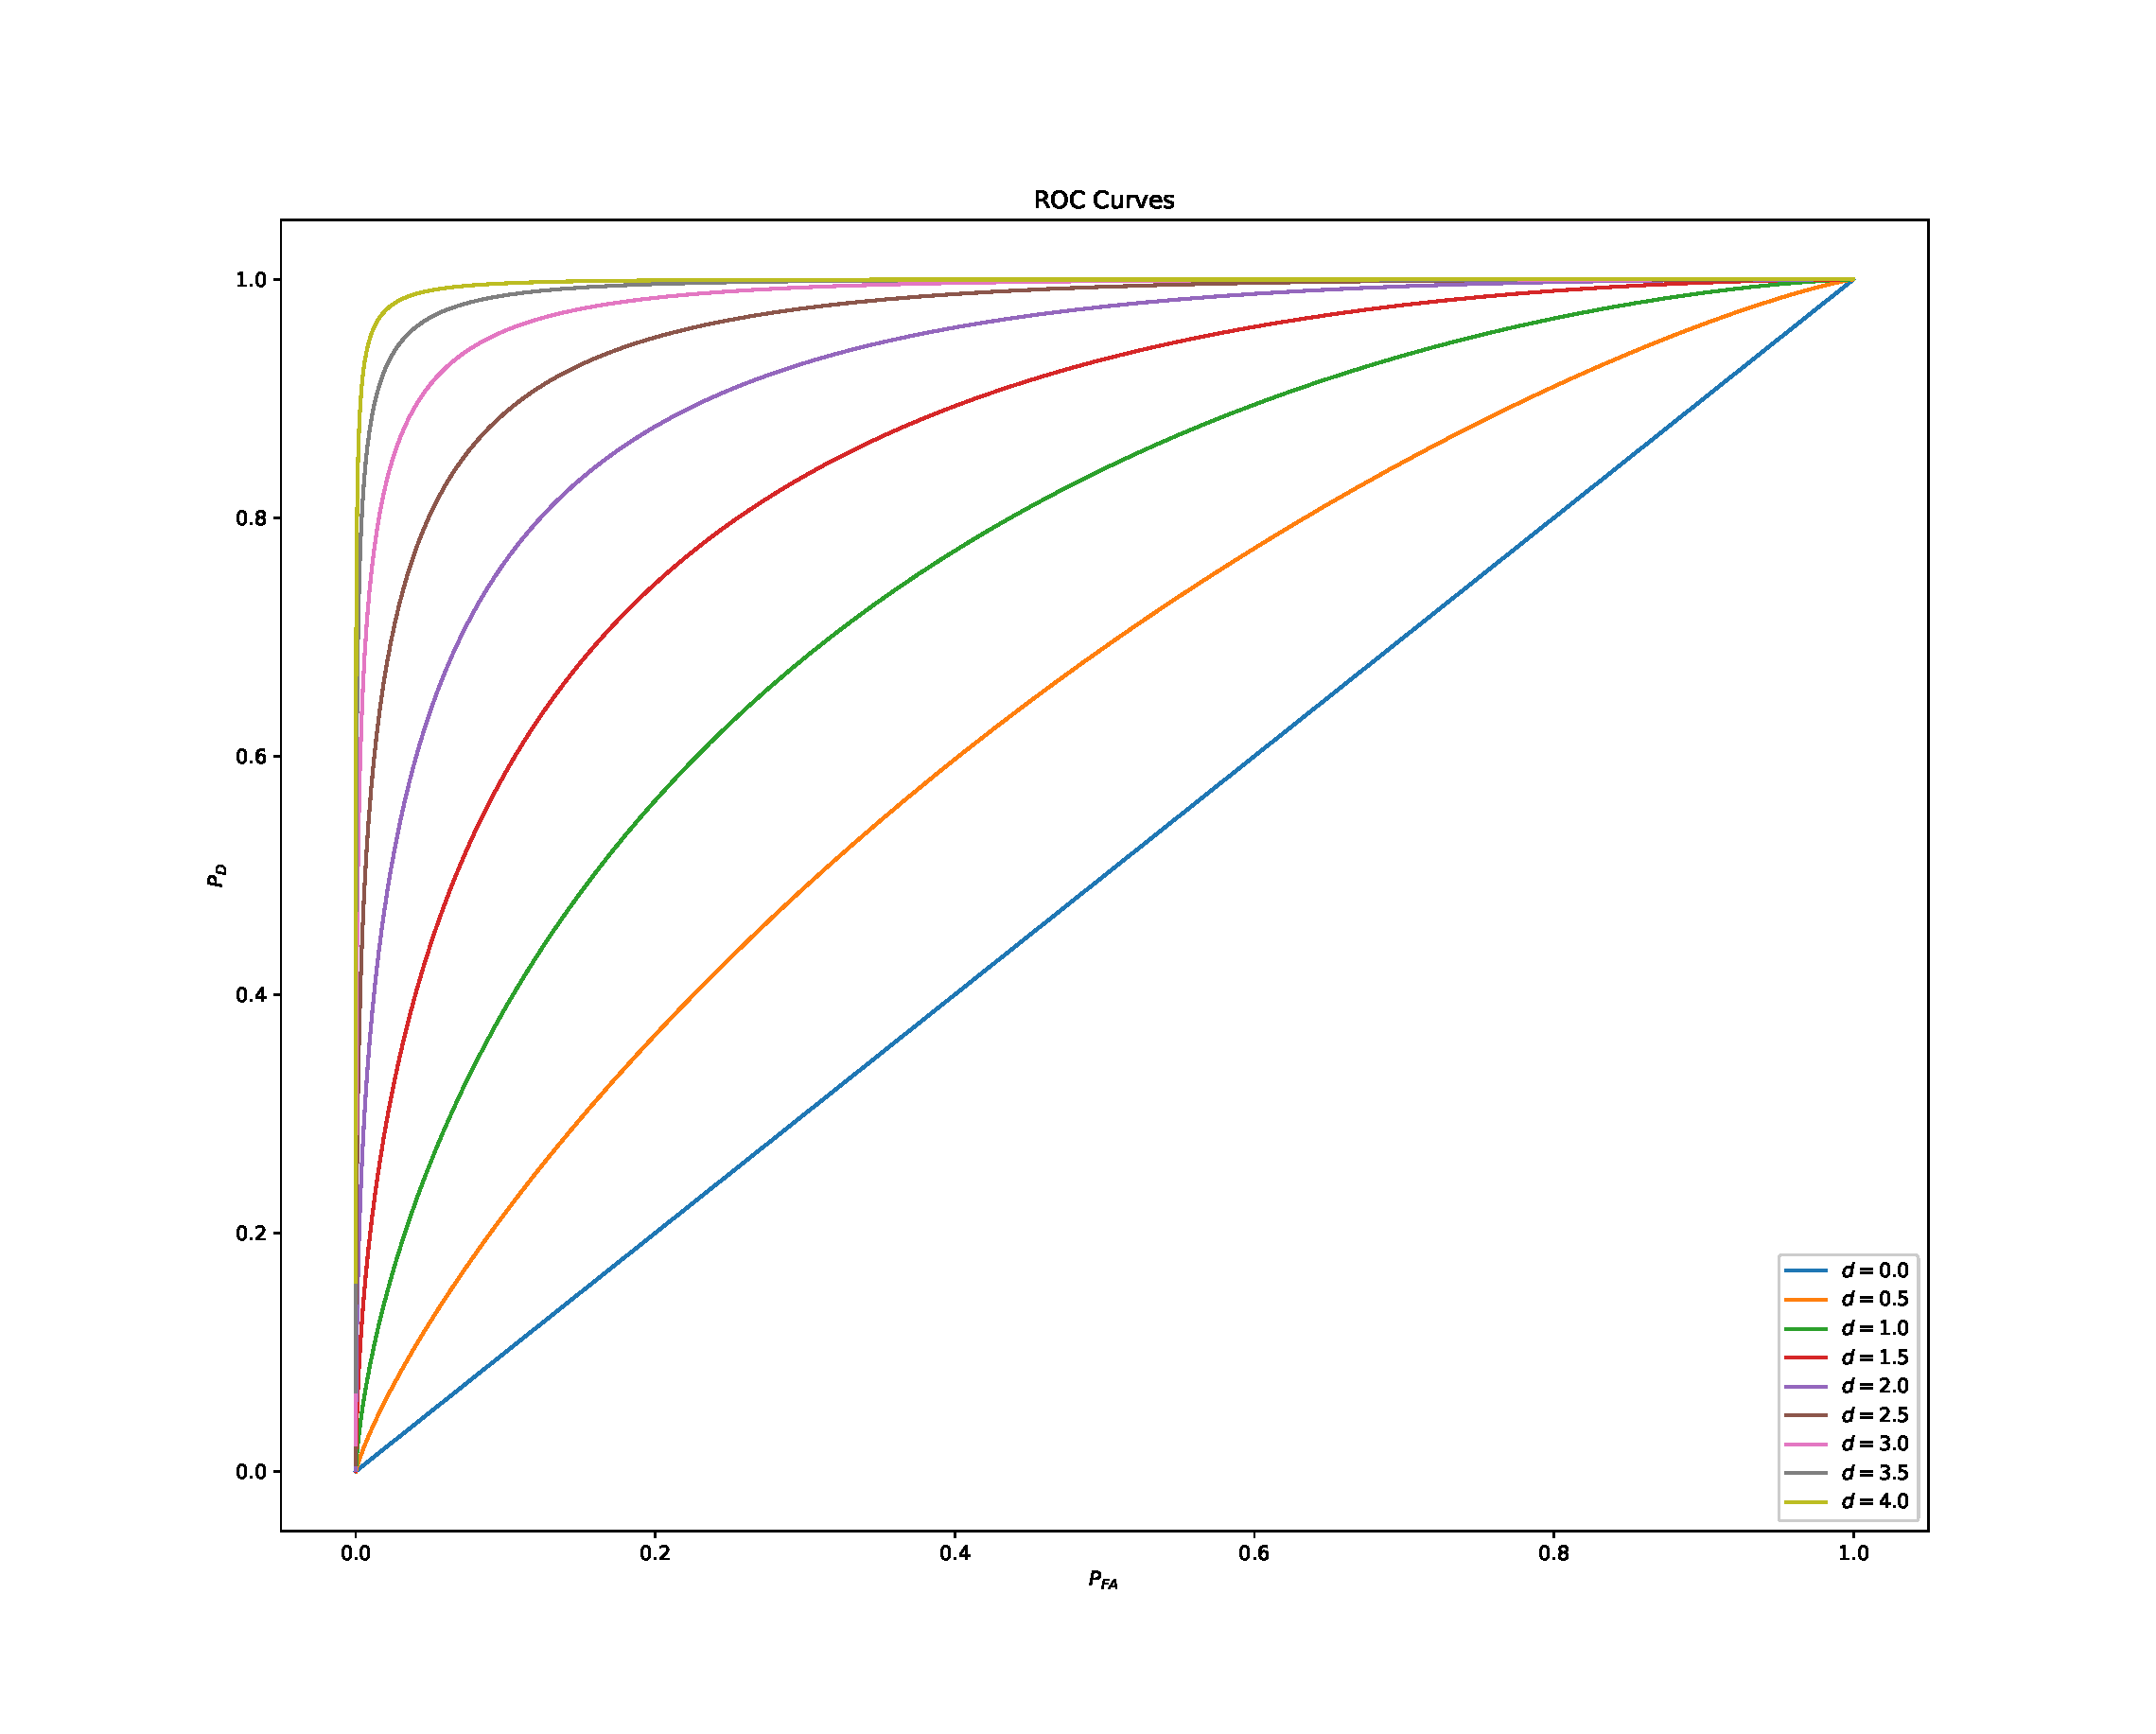
\includegraphics[scale=0.5]{hw5-1-1.eps}
\end{center}
\end{figure}

I found the $d$ required to acheive $P_{FA} < 0.01$ and $P_{D} > 0.99$ to be $d = 4.67$


\end{document}

